\apendice{Documentación de usuario} \label{apendice:usuario}

\section{Introducción}

En esta sección se recogen los requisitos que requiere nuestra aplicación, así como los detalles para la instalación y uso de la misma por el usuario final\footnote{\, Por ahora, no se incluyen los detalles referentes a la versión de escritorio, dado que el soporte de Flutter para estas plataformas está aún en fase \emph{alfa} \cite{flutter-desktop}.}.

\section{Requisitos de usuarios}

Para la versión \textbf{Android}, se deben cumplir los siguientes requisitos:

\vspace{-0.3cm}
\begin{itemize} [\textbullet]
	\item Mínimo 18 MB de espacio de almacenamiento libre. El paquete de instalación tiene un tamaño de 6,3 MB, y una vez instalada ocupa 16,36 MB. No obstante, ese tamaño aumentará ligeramente según se vayan almacenando resúmenes.
	
	\item Versión de Android igual o superior a la 4.1 (\emph{JellyBean} - API 16).
\end{itemize}

En el caso de \textbf{iOS}:

\vspace{-0.3cm}
\begin{itemize} [\textbullet]
	\item Mínimo 20 MB de espacio de almacenamiento libre. En este caso, el peso del paquete es de 6,9 MB, y una vez instalada ocupa 17,2 MB.
	
	\item Versión de iOS 8 o superior.
\end{itemize}

\newpage

Y en el caso de la versión \emph{\textbf{web}}:

\begin{itemize} [\textbullet]
	\item Los navegadores \emph{web} soportados son Google Chrome\footnote{Hemos probado la \emph{app} en navegadores basados en Chromium, como Brave, y también parecen funcionar.}, Mozilla Firefox, Safari o Edge.
\end{itemize}

En todos los casos se requiere conexión a Internet para generar nuevos resúmenes (los resúmenes ya generados se pueden consultar \emph{offline}). La \emph{app} de JIZT no requiere de permisos adicionales en ninguna de las plataformas.

La aplicación solo está disponible por el momento en inglés, dado que este es el único lenguaje soportado actualmente por el servicio de generación de resúmenes.

\vspace{2cm}

\section{Instalación}

En esta sección detallamos el proceso de instalación en las diferentes plataformas.

\subsection{Android}

\subsubsection{Instalación recomendada}

Se recomienda que el usuario instale la aplicación desde Google Play.

Para ello, simplemente basta con buscar la aplicación <<JIZT AI Summarization>> y pulsar en <<Instalar>>.

\newpage

\begin{figure}[H]
	\centering
	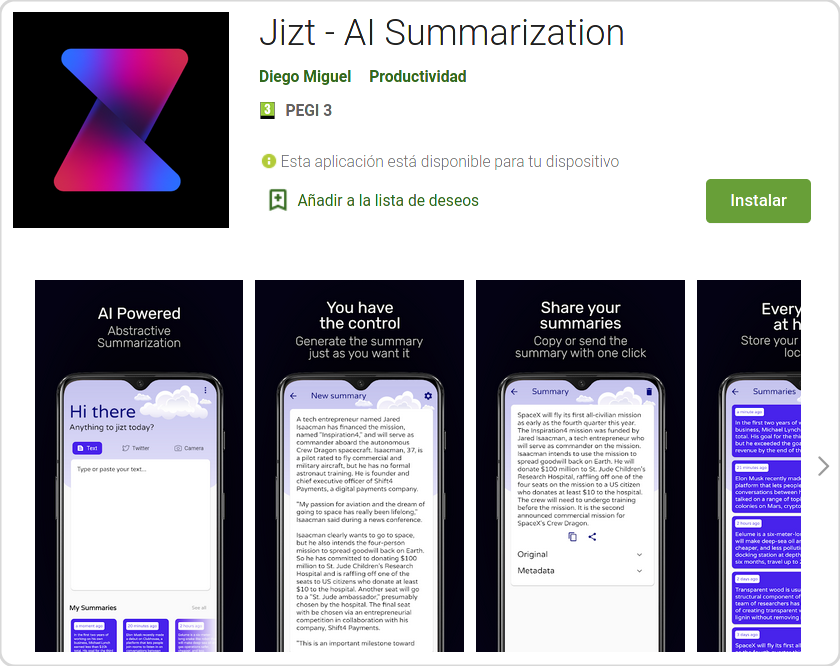
\includegraphics[width=0.8\textwidth]{jizt-google-play}
	\caption{Instalar JIZT desde Google Play.}
\end{figure}

\subsection{iOS}

Por el momento, la aplicación no ha sido publicada en la App Store, e iOS no proporciona ninguna manera oficial para la instalación de aplicaciones desde fichero\footnote{\, Como aclaración al margen de Manual de Usuario, la aplicación no ha sido publicada en la App Store por su elevado precio (99\$ al año por la cuenta de desarrollador, frente a los 25\$ de por vida, en el caso de Play Store).}.

Por tanto, se recomienda a los usuarios que accedan desde su navegador móvil a la versión \emph{web} de JIZT (ver siguiente sección).

\subsection{\emph{Web}}

Se puede acceder a la aplicación directamente a través de \href{https://dmlls.github.io/jizt-tfg-app}{app.jizt.it}, sin ser necesario realizar ninguna instalación.

\newpage

\section{Manual del usuario}

Una vez instalada la aplicación, el usuario está en disposición de comenzar a utilizarla. El funcionamiento en interfaz de la aplicación en las diferentes plataformas es homogéneo, por lo que todo lo explicado a continuación es válido para cualquiera de ellas.

\subsection{Generar un nuevo resumen} \label{subsection:nuevo-resumen}

La generación de resúmenes se trata de una de las funciones principales de la aplicación.

Los pasos que debemos seguir para generar un nuevo resumen son los siguientes:

\begin{enumerate}
	\item En la pantalla de inicio, pulsar sobre el campo de texto central, el cual contiene escrito <<\emph{Type or paste your text}>> (en español, <<Escribe o pega tu texto>>).
	
	\item Escribir el texto o pulsar en el icono de la esquina superior derecha, el sirve para pegar el texto desde el portapapeles.
	
	\item Pulsar en <<\emph{Summarize}>> (<<resumir>>).
	
	\item Se mostrará una barra que simboliza que el resumen está siendo generado.
	
	\item Una vez completado el resumen, se mostrará una nueva pantalla con el resumen.
\end{enumerate}

Se puede visualizar un vídeo que recoge el proceso en \href{https://github.com/dmlls/jizt-tfg/blob/main/docs/video-tutorials/1-generar-nuevo-resumen.mp4}{https://github.com/\newline dmlls/jizt-tfg/blob/main/docs/video-tutorials/1-generar-nuevo-resumen.mp4}.

\subsection{Ajustar la longitud del resumen a generar}

JIZT nos permite establecer la longitud deseada del resumen generado. Esta longitud se establece como un porcentaje de la longitud del texto original.

Para ajustar la longitud del resumen que vamos a generar, debemos seguir los dos primeros pasos indicados en la sección <<\hyperref[subsection:nuevo-resumen]{Generar un nuevo resumen}>>.

Una vez en la pantalla de nuevo resumen, podemos ajustar el \emph{slider} que aparece en la parte inferior de la pantalla, estableciendo la longitud mínima y máxima de nuestro resumen.

Se puede visualizar un vídeo que recoge el proceso en \href{https://github.com/dmlls/jizt-tfg/blob/main/docs/video-tutorials/2-ajustar-longitud.mp4}{https://github.com/\newline dmlls/jizt-tfg/blob/main/docs/video-tutorials/2-ajustar-longitud.mp4}.

\subsection{Ver todos los resúmenes generados}

La aplicación muestra en la pantalla principal una vista previa de los últimos resúmenes generados en forma de lista deslizable. Pulsando sobre cualquiera de ellos, se accede a los detalles del mismo.

Si se quieren ver todos los resúmenes, se puede pulsar en <<\emph{See all}>> (<<ver todos>>). Se mostrará una nueva pantalla en la que aparece una lista con todos los resúmenes, ordenados temporalmente de más recientes a más antiguos. Se puede pulsar sobre cualquiera de ellos para obtener más detalles.

Se puede visualizar un vídeo que recoge el proceso en \href{https://github.com/dmlls/jizt-tfg/blob/main/docs/video-tutorials/3-ver-todos-resúmenes.mp4}{https://github.com/\newline dmlls/jizt-tfg/blob/main/docs/video-tutorials/3-ver-todos-resúmenes.mp4}.

\subsection{Borrar un resumen} \label{subsection:borrar}

Para borrar un resumen, se puede pulsar en el símbolo que aparece en la esquina superior derecha en la pantalla de <<\emph{Summary}>> (resumen).

Se puede acceder a esta pantalla de tres formas diferentes:

\begin{enumerate}
	\item Tras generar un resumen, se muestra dicha pantalla por defecto.
	
	\item Haciendo \emph{click} en cualquiera de los resúmenes que aparecen en la parte inferior de la pantalla principal.
	
	\item Pulsando en <<\emph{See all}>> (<<ver todos>>) y haciendo \emph{click} en cualquiera de los resúmenes.
\end{enumerate}

Se puede visualizar un vídeo que recoge el proceso en \href{https://github.com/dmlls/jizt-tfg/blob/main/docs/video-tutorials/4-borrar-resumen.mp4}{https://github.com/\newline dmlls/jizt-tfg/blob/main/docs/video-tutorials/4-borrar-resumen.mp4}.

\subsection{Copiar un resumen}

Para copiar un resumen, se debe estar en la pantalla de <<\emph{Summary}>> (resumen). Para acceder a esta pantalla, seguir cualquiera de las alternativas listadas en la sección ``\hyperref[subsection:borrar]{Borrar un resumen}''.

Una vez en esta pantalla, se debe pulsar en el siguiente icono:

Tras pulsar dicho icono, el texto se habrá copiado al portapapeles de nuestro dispositivo.

Se puede visualizar un vídeo que recoge el proceso en \href{https://github.com/dmlls/jizt-tfg/blob/main/docs/video-tutorials/5-copiar-resumen.mp4}{https://github.com/\newline dmlls/jizt-tfg/blob/main/docs/video-tutorials/5-copiar-resumen.mp4}.

\subsection{Compartir un resumen}

Para copiar un resumen, se debe estar en la pantalla de <<\emph{Summary}>> (resumen). Para acceder a esta pantalla, seguir cualquiera de las alternativas listadas en la sección ``\hyperref[subsection:borrar]{Borrar un resumen}''.

Una vez en esta pantalla, se debe pulsar en el siguiente icono:

A continuación, se mostrará una lista de aplicaciones a través de las cuales se puede compartir el resumen.

Se puede visualizar un vídeo que recoge el proceso en \href{https://github.com/dmlls/jizt-tfg/blob/main/docs/video-tutorials/6-compartir-resumen.mp4}{https://github.com/\newline dmlls/jizt-tfg/blob/main/docs/video-tutorials/6-compartir-resumen.mp4}.

\subsection{Ver el texto a partir del cual se generó un resumen}

Para ver el texto original de un resumen, se debe estar en la pantalla de <<\emph{Summary}>> (resumen). Para acceder a esta pantalla, seguir cualquiera de las alternativas listadas en la sección <<\hyperref[subsection:borrar]{Borrar un resumen}>>.

Una vez en dicha pantalla, se debe pulsar sobre <<\emph{Original}>>.

Se puede visualizar un vídeo que recoge el proceso en \href{https://github.com/dmlls/jizt-tfg/blob/main/docs/video-tutorials/7-ver-original.mp4}{https://github.com/\newline dmlls/jizt-tfg/blob/main/docs/video-tutorials/7-ver-original.mp4}.

\subsection{Obtener más información acerca de un resumen}

Para obtener más información de un resumen, se debe estar en la pantalla de <<\emph{Summary}>> (resumen). Para acceder a esta pantalla, seguir cualquiera de las alternativas listadas en la sección <<\hyperref[subsection:borrar]{Borrar un resumen}>>.

Una vez en dicha pantalla, se debe pulsar sobre <<\emph{More info}>> (<<Más información>>).

Se puede visualizar un vídeo que recoge el proceso en \href{https://github.com/dmlls/jizt-tfg/blob/main/docs/video-tutorials/8-m\%C3\%A1s-info.mp4}{https://github.com/\newline dmlls/ jizt-tfg/blob/main/docs/video-tutorials/8-m\%C3\%A1s-info.mp4}.

\subsection{Generar un resumen a partir de un documento}

Por el momento, esta opción no está disponible. No obstante, pronto será implementada.

\subsection{Generar un resumen a partir de una imagen}

Por el momento, esta opción no está disponible. No obstante, pronto será implementada.